\documentclass{article}

\usepackage[utf8]{inputenc}
\usepackage{amsmath}
\usepackage{algpseudocode}

\usepackage{algorithm}
\usepackage{graphicx}
\usepackage[justification=centering]{caption}

\algnewcommand\algorithmicforeach{\textbf{parallel for each}}
\algdef{S}[FOR]{ForEach}[1]{\algorithmicforeach\ #1\ \algorithmicdo}


\title{Induced 6-Cycle Counting in Bipartite Networks}

\begin{document}

\maketitle

\begin{abstract}
Finding subgraphs in bipartite networks is integral to understanding its underlying structure. The smallest cycle in a bipartite network is a 4-cycle, which is also known as a butterfly. Previous works have developed efficient butterfly counting algorithms. In this paper, we propose a parallel algorithm for efficiently counting induced 6-cycles.
\end{abstract}

\section{Introduction}
In unipartite graphs, the smallest cycle is a 3-cycle, which is also known as a triangle. In bipartite graphs, triangles do not exist. The smallest non-trivial subgraph in a bipartite graph is a 4-cycle, which is also known as a butterfly.

\begin{figure}[h]
    \centering
    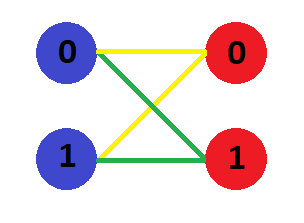
\includegraphics[width=0.25\textwidth]{figures/Butterfly.png}
    \caption{\small This graph depicts a butterfly. Nodes in u are in blue while nodes in v are in red. The butterfly is made of two wedges, which are highlighted in yellow and green.}
    \label{fig:butterfly}
\end{figure}

Recent algorithms for butterfly counting use the concept of combining wedges (2-paths) to count butterflies (see Figure 1).


\begin{figure}[h]
    \centering
    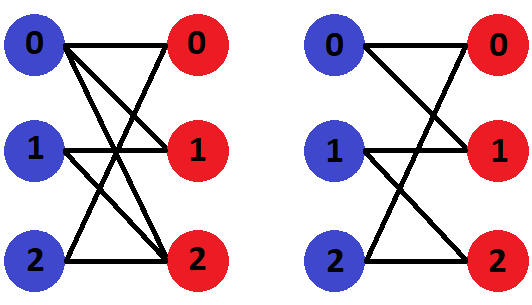
\includegraphics[width=0.25\textwidth]{figures/Induced vs Noninduced.png}
    \caption{\small The graph on the left depicts a non-induced 6-cycle. The graph on the right depicts an induced 6-cycle. Nodes in u are in blue while nodes in v are in red. In the non-induced graph, the removal of the edge from u0 to v2 won't affect the 6-cycle.}
    \label{fig:induced}
\end{figure}

Given the relevance of bipartite graphs in real-world relationships, it is desirable to find larger motifs within these graphs. This paper presents a framework for counting induced 6-cycles (see Figure 2) in bipartite graphs which uses the affordances of parallization to maximize efficiency.

\section{Notation}
We work on a simple bipartite graph 
\textit{G = (U, V, E)} where U is the set of nodes in the left set, V is the set of nodes in right set, and E is the set of edges.
An induced 6-cycle is a set of six nodes \textit{u1, u2, u3} $\in$ \textit{U} and \textit{v1, v2, v3} $\in$ \textit{V} such that its internal edges exactly form a cycle.
\\
\begin{algorithm}[H]
\caption{Par6CycleCount(\textit{G})}
\hspace*{\algorithmicindent} \textbf{Input:} \textit{G}: graph \\
\hspace*{\algorithmicindent} \textbf{Output:} \textit{c}: count of induced 6-cycles
\begin{algorithmic}[1]
    \State $W \gets $list of wedges $(u1 \rightarrow v1 \rightarrow u2)$
    \State $c \gets $0
    \ForEach {$w \in W$}
        \State BFS on $u2$ until depth 4 $(u2 \rightarrow v2 \rightarrow u3 \rightarrow v3 \rightarrow u4)$ and if $u1 = u3$, $v1 = v3$ or $u2 = u4$, skip $w$
        \ForEach {$u4 \in$ depth 4}
            \If{$u4 = u1$}
                \State $c \gets c + 1$
            \EndIf
        \EndFor
    \EndFor
\end{algorithmic}
\end{algorithm}


\end{document}